\subsection*{Lösungen zu Kapitel~\ref{kapitel:Inversion}: \emph{Inversion am Kreis}}

\begin{figure}[ht]
	\centering
	\begin{tabularx}{\textwidth}{X c X c X}
		& 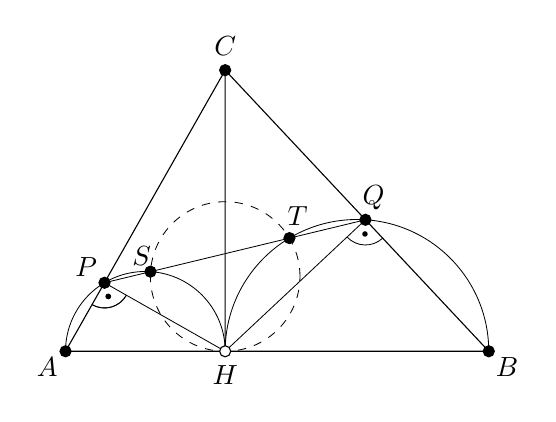
\begin{tikzpicture}[x=1.25cm,y=1.25cm]
			\draw [line width=0.3, shift={(-0.811,0)}] (0:0.811) arc (0:180:0.811);
			\draw [line width=0.3, shift={(1.339,0)}] (0:1.339) arc (0:180:1.339);
			\draw [dashed,line width=0.3] (0,0.76) circle (0.76);
			\coordinate (A) at (-1.622,0);
			\coordinate (B) at (2.678,0);
			\coordinate (C) at (0,2.856);
			\coordinate (H) at (0,0);
			\coordinate (P) at (-1.226,0.696);
			\coordinate (Q) at (1.425,1.336);
			\coordinate (S) at(-0.759,0.809);
			\coordinate (T) at (0.653,1.15);
			\draw (C) to (A) to (B) to (C) to (H);
			\draw [line width=0.3] (H) to (P) to (Q) to cycle;
			\draw [line width=0.3,shift={(P)}] (240.412:0.32cm) arc (240.412:330.412:0.32cm);
			\fill [shift={(P)}] (285.412:0.18cm) circle (1pt);
			\draw [line width=0.3,shift={(P)}] (240.412:0.32cm) arc (240.412:330.412:0.32cm);
			\fill [shift={(P)}] (285.412:0.18cm) circle (1pt);
			\draw [line width=0.3,shift={(Q)}] (223.16:0.32cm) arc (223.16:313.16:0.32cm);
			\fill [shift={(Q)}] (268.16:0.18cm) circle (1pt);
			\draw[fill=black] (A) circle (2pt) node[shift={(220:2ex)}] {$A$};
			\draw[fill=black] (B) circle (2pt) node[shift={(-40:2ex)}] {$B$};
			\draw[fill=black] (C) circle (2pt) node[shift={(90:2ex)}] {$C$};
			\draw[fill=white] (H) circle (2pt) node[shift={(-90:2ex)}] {$H$};
			\draw[fill=black] (P) circle (2pt) node[shift={(140:2ex)}] {$P$};
			\draw[fill=black] (Q) circle (2pt) node[shift={(70:2ex)}] {$Q$};
			\draw[fill=black] (S) circle (2pt) node[shift={(120:1.5ex)}] {$S$};
			\draw[fill=black] (T) circle (2pt) node[shift={(70:2ex)}] {$T$};
		\end{tikzpicture} & & 
		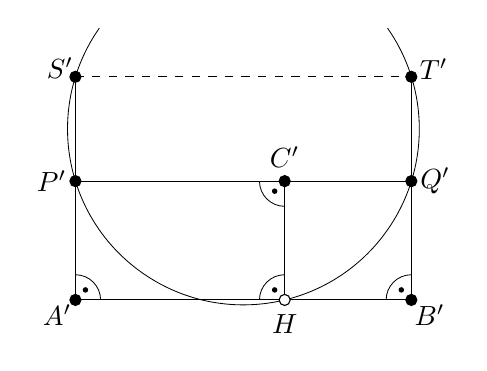
\begin{tikzpicture}[x=1.25cm,y=1.25cm]
			\draw [line width=0.3, shift={(-0.419,1.737)}] (145:1.787) arc (145:395:1.787);
			\coordinate (A) at (-2.126,0);
			\coordinate (B) at (1.287,0);
			\coordinate (C) at (0,1.207);
			\coordinate (H) at (0,0);
			\coordinate (P) at (-2.126,1.207);
			\coordinate (Q) at (1.287,1.207);
			\coordinate (S) at(-2.126,2.267);
			\coordinate (T) at (1.287,2.267);
			\draw (S) to (A) to (B) to (T);
			\draw (P) to (Q);
			\draw [line width=0.3,dashed] (S) to (T);
			\draw (C) to (H);
			\draw [line width=0.3,shift={(H)}] (90:0.32cm) arc (90:180:0.32cm);
			\fill [shift={(H)}] (135:0.18cm) circle (1pt);
			\draw [line width=0.3,shift={(C)}] (180:0.32cm) arc (180:270:0.32cm);
			\fill [shift={(C)}] (225:0.18cm) circle (1pt);
			\draw [line width=0.3,shift={(A)}] (0:0.32cm) arc (0:90:0.32cm);
			\fill [shift={(A)}] (45:0.18cm) circle (1pt);
			\draw [line width=0.3,shift={(B)}] (90:0.32cm) arc (90:180:0.32cm);
			\fill [shift={(B)}] (135:0.18cm) circle (1pt);
			\draw[fill=black] (A) circle (2pt) node[shift={(220:2ex)}] {$A'$};
			\draw[fill=black] (B) circle (2pt) node[shift={(-40:2ex)}] {$B'$};
			\draw[fill=black] (C) circle (2pt) node[shift={(90:2ex)}] {$C'$};
			\draw[fill=white] (H) circle (2pt) node[shift={(-90:2ex)}] {$H$};
			\draw[fill=black] (P) circle (2pt) node[shift={(180:2ex)}] {$P'$};
			\draw[fill=black] (Q) circle (2pt) node[shift={(0:2ex)}] {$Q'$};
			\draw[fill=black] (S) circle (2pt) node[shift={(150:1.5ex)}] {$S'$};
			\draw[fill=black] (T) circle (2pt) node[shift={(20:2ex)}] {$T'$};
		\end{tikzpicture} & \\
		& vor Inversion & & nach Inversion & 
	\end{tabularx}
\end{figure}

\begin{proof}[Lösung zu Aufgabe~\ref{aufgabe:450943} \textmd{(\href{https://www.mathematik-olympiaden.de/moev/index.php?option=com_download&thema=a&format=raw&datei=A45094a.pdf}{MO 450943})}]
	Wir invertieren an~$H$. Die Bildpunkte werden wie üblich mit $A'$,~$B'$,~\ldots\ bezeichnet. Wegen $\winkel APH=90^\circ=\winkel HPC$ gilt $\winkel HA'P'=90^\circ= \winkel P'C'H$ nach Eigenschaft~\ref{itm:Winkel}. Weil die Geraden $CH$ und~$AB$ durch~$H$ gehen, werden sie auf sich selbst abgebildet. Also steht $C'H$ immer noch senkrecht auf~$A'B'$. Folglich ist $A'HC'P'$ ein Rechteck. Analog ist $HB'Q'C'$ ein Rechteck. Also ist auch $A'B'Q'P'$ ein Rechteck. Weil $S$ auf dem Umkreis $\odot AHP$ liegt, muss $S'$ auf der Geraden~$A'P'$ liegen. Analog liegt $T'$ auf~$B'Q'$. Weil schließlich $S$~und~$T$ auf~$PQ$ liegen, müssen $S'$~und~$T'$ auf dem Umkreis $\odot P'HQ'$ liegen. Nach Satz vom Sehnenviereck gilt dann $\winkel P'S'T'=180^\circ-\winkel T'Q'P'=180^\circ-90^\circ=90^\circ$. Also ist auch $P'Q'T'S'$ ein Rechteck. Folglich ist $S'T'$ parallel zu~$A'B'$. Das bedeutet aber genau, dass vor der Inversion der Umkreis $\odot HTS$ die Gerade~$AB$ in~$H$ berührt haben muss.
\end{proof}

\begin{proof}[Lösung zu Aufgabe~\ref{aufgabe:IMO1996} \textmd{(\href{https://artofproblemsolving.com/community/c3823_1996_imo}{IMO 1996/2})}]
	Seien $X$~und~$Y$ die Schnittpunkte der Winkelhalbierenden von $\winkel PBA$ und $\winkel ACP$ mit~$AP$.
	% Tien: Vielleicht ein "bzw.\" oder "respektive".
	Wir wollen $X=Y$ zeigen. Dazu invertieren wir an~$A$. Wie üblich werden die Bildpunkte unter der Inversion mit $B'$,~$C'$,~\ldots\ bezeichnet. Aus Eigenschaft~\ref{itm:Winkel} folgt dann $\winkel P'B'C'=\winkel P'B'A'-\winkel C'B'A'=\winkel APB-\winkel ACB$ und analog $\winkel B'C'P=\winkel CPA-\winkel CBA$. Die seltsame Winkelbedingung aus der Aufgabenstellung sagt uns also genau, dass das Dreieck $C'B'P'$ gleichschenklig ist.
	\begin{figure}[ht]
		\centering
		\begin{tabularx}{\textwidth}{X c X c X}
			& 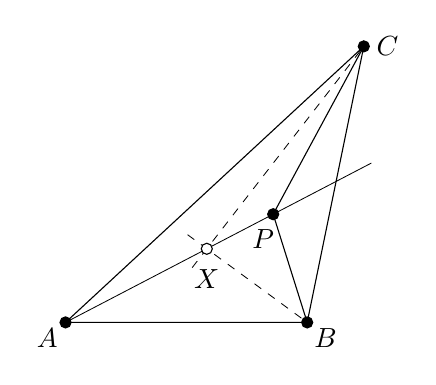
\begin{tikzpicture}
				\coordinate (A) at (0,0);
				\coordinate (B) at (3.069,0);
				\coordinate (C) at (3.788,3.506);
				\coordinate (P) at (2.637,1.374);
				\coordinate (X) at (1.794,0.935);
				\coordinate (Q) at (1.425,1.336);
				\draw (C) to (A) to (B) to (P) to (C) to (B);
				\draw [line width=0.3, shorten >=-4em] (A) to (P);
				\draw [line width=0.3, dashed, shorten <=-2ex] (X) to (B);
				\draw [line width=0.3, dashed, shorten <=-2ex] (X) to (C);
				\draw[fill=black] (A) circle (2pt) node[shift={(220:2ex)}] {$A$};
				\draw[fill=black] (B) circle (2pt) node[shift={(-40:2ex)}] {$B$};
				\draw[fill=black] (C) circle (2pt) node[shift={(0:2ex)}] {$C$};
				\draw[fill=black] (P) circle (2pt) node[shift={(-112:2.25ex)}] {$P$};
				\draw[fill=white] (X) circle (2pt) node[shift={(270:2.5ex)}] {$X$};
			\end{tikzpicture} & & 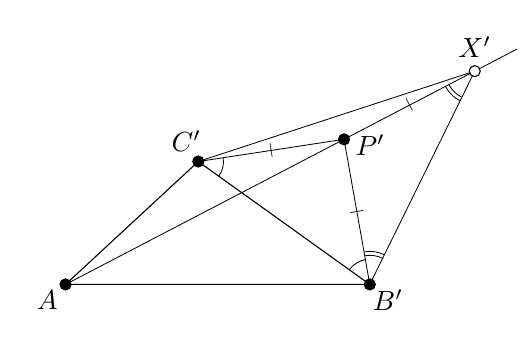
\begin{tikzpicture}
				\coordinate (A) at (0,0);
				\coordinate (B) at (3.864,0);
				\coordinate (C) at (1.686,1.561);
				\coordinate (P) at (3.537,1.843);
				\coordinate (X) at (5.197,2.709);
				\draw (A) to (B) to (C) to cycle;
				\draw [line width=0.3,shorten >=-4ex] (P) to node[pos=0.5, sloped] {$\scriptscriptstyle|$} (X);
				\draw [line width=0.3] (A) to (P);
				\draw [line width=0.3] (C) to node[pos=0.5, sloped] {$\scriptscriptstyle|$} (P);
				\draw [line width=0.3] (P) to node[pos=0.5, sloped] {$\scriptscriptstyle|$} (B);
				\draw [line width=0.3] (C) to (X) to (B);
				\draw [line width=0.3,shift={(B)}] (100.056:0.32cm) arc (100.056:144.372:0.32cm);
				\draw [line width=0.3,shift={(C)}] (324.372:0.32cm) arc (324.372:368.688:0.32cm);
				\draw [line width=0.3,shift={(B)}] (63.793:0.42cm) arc (63.793:100.056:0.42cm);
				\draw [line width=0.3,shift={(B)}] (63.793:0.37cm) arc (63.793:100.056:0.37cm);
				\draw [line width=0.3,shift={(X)}] (207.53:0.42cm) arc (207.53:243.793:0.42cm);
				\draw [line width=0.3,shift={(X)}] (207.53:0.37cm) arc (207.53:243.793:0.37cm);
				\draw[fill=black] (A) circle (2pt) node[shift={(220:2ex)}] {$A$};
				\draw[fill=black] (B) circle (2pt) node[shift={(-40:2ex)}] {$B'$};
				\draw[fill=black] (C) circle (2pt) node[shift={(120:2ex)}] {$C'$};
				\draw[fill=black] (P) circle (2pt) node[shift={(-12:2.25ex)}] {$P'$};
				\draw[fill=white] (X) circle (2pt) node[shift={(90:2ex)}] {$X'$};
			\end{tikzpicture}
			& \\
			& vor Inversion & & nach Inversion & 
		\end{tabularx}
	\end{figure}
	
	Als nächstes untersuchen wir, wohin $X$ unter der Inversion geschickt wird. Weil $X$ auf~$AP$ liegt, liegt $X'$ auf der Geraden~$AP'$. Wir können sogar genauer sagen, dass $P'$ zwischen $A$~und~$X'$ liegt, weil vor der Inversion $X$ zwischen $A$~und~$P$ lag. Vor der Inversion galt $\winkel XBA=\frac12\winkel PBA$. Aus Eigenschaft~\ref{itm:Winkel} folgt also $\winkel AX'B'=\frac 12\winkel AP'B'$. Nach dem Außenwinkelsatz im Dreieck $P'B'X'$ gilt zudem $\winkel AP'B'=\winkel AX'B'+\winkel X'B'P'$. Also muss auch $\winkel X'B'P'=\frac 12\winkel AP'B'$ gelten. Folglich ist auch das Dreieck $P'B'X'$ gleichschenklig und wir erhalten $\abs{X'P'}=\abs{B'P'}=\abs{C'P'}$. Mit der gleichen Argumentation folgt auch $\abs{Y'P'}=\abs{B'P'}=\abs{C'P'}$, also $\abs{X'P'}=\abs{Y'P'}$. Wie wir bereits gesehen haben, liegen $X'$~und~$Y'$ auf der gleichen Seite von~$P'$. Also muss $X'=Y'$ sein. Es folgt $X=Y$, wie gewünscht.
\end{proof}

\begin{proof}[Lösung zu Aufgabe~\ref{aufgabe:521243} \textmd{(\href{https://www.mathematik-olympiaden.de/moev/index.php?option=com_download&thema=a&format=raw&datei=A52124a.pdf}{MO 521243})}]
	Bei dieser Aufgabe bringt es wenig, am gewünschten Berührpunkt zu invertieren, denn wir wissen ja (noch) gar nicht, wo der liegt. Stattdessen invertieren wir an~$X$. Überlegt euch zunächst selbst, wie die Skizze nach der Inversion aussieht (bzw.\ warum sie so wie unten aussieht)~-- ihr werdet feststellen, dass sich durch die Inversion eigentlich nichts geändert hat. Auf den ersten Blick wirkt es also, als hätten wir nichts erreicht. Auf den zweiten Blick haben wir jedoch durch diese Feststellung die Aufgabe schon fast gelöst!
	\begin{figure}[ht]
		\centering
		\begin{tabularx}{\textwidth}{X c X c X}
			& 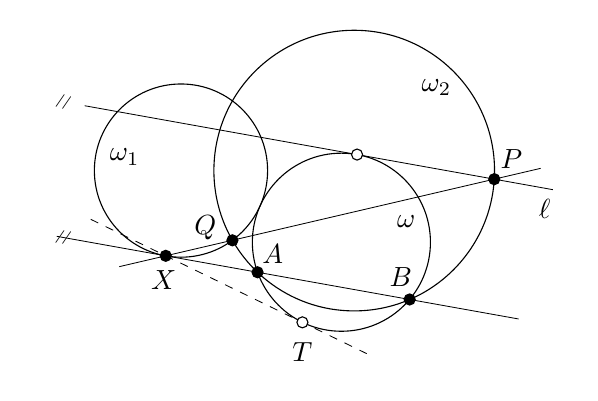
\begin{tikzpicture}[x=1.1cm,y=1.1cm]
				\clip (-1.77,-2.33) rectangle (4.49,1.65);
				\draw (0,0) circle (1);
				\draw (2,0) circle (1.62);
				\draw (1.852,-0.827) circle (1.028);
				\coordinate (Q) at (0.594,-0.805);
				\coordinate (X) at (-0.176,-0.984);
				\coordinate (P) at (3.617,-0.099);
				\coordinate (A) at (0.884,-1.174);
				\coordinate (B) at (2.64,-1.488);
				\coordinate (T) at (1.402,-1.752);
				\coordinate (D) at (2.033,0.185);
				\coordinate (E) at (0.913,-0.408);
				\draw [line width=0.3,shorten <=-4ex,shorten >=-4ex] (X) to (P);
				\draw [line width=0.3,shorten <=-4em,shorten >=-4em] (X) to node [pos=-0.42,sloped] {$\scriptscriptstyle/\!/$} (B);
				\draw [line width=0.3,shorten <=-5ex,shorten >=-10em] (P) to node [pos=3.14,sloped] {$\scriptscriptstyle/\!/$} (D);
				\draw [line width=0.3,dashed,shorten <=-7ex,shorten >=-6ex] (X) to (T);
				\draw[fill=black] (A) circle (2pt) node[shift={(50:2ex)}] {$A$};
				\draw[fill=black] (B) circle (2pt) node[shift={(112:2ex)}] {$B$};
				\draw[fill=black] (P) circle (2pt) node[shift={(50:2.25ex)}] {$P$};
				\draw[fill=black] (Q) circle (2pt) node[shift={(155:2.5ex)}] {$Q$};
				\draw[fill=black] (X) circle (2pt) node[shift={(265:2ex)}] {$X$};
				\draw[fill=white] (T) circle (2pt) node[shift={(270:2.5ex)}] {$T$};
				\draw[fill=white] (D) circle (2pt);
				\node[shift={(270:2.5ex)}] at (-0.65,0.5) {$\omega_1$};
				\node[shift={(270:2.5ex)}] at (2.95,1.3) {$\omega_2$};
				\node[shift={(270:2.5ex)}] at (2.6,-0.25) {$\omega$};
				\node[shift={(270:2.5ex)}] at (4.2,-0.1) {$\ell$};
			\end{tikzpicture} & & 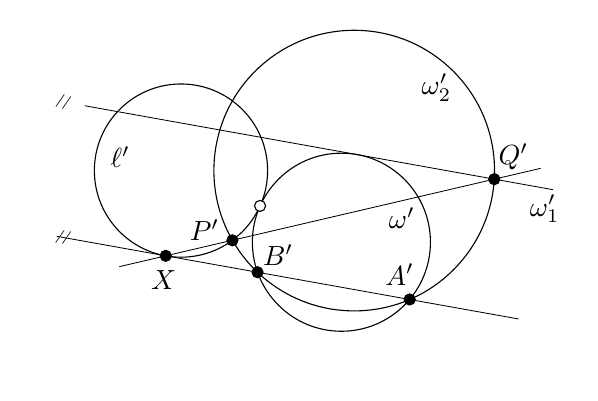
\begin{tikzpicture}[x=1.1cm,y=1.1cm]
				\clip (-1.77,-2.33) rectangle (4.49,1.65);
				\draw (0,0) circle (1);
				\draw (2,0) circle (1.62);
				\draw (1.852,-0.827) circle (1.028);
				\coordinate (Q) at (0.594,-0.805);
				\coordinate (X) at (-0.176,-0.984);
				\coordinate (P) at (3.617,-0.099);
				\coordinate (A) at (0.884,-1.174);
				\coordinate (B) at (2.64,-1.488);
				\coordinate (D) at (2.033,0.185);
				\coordinate (E) at (0.913,-0.408);
				\coordinate (T) at (1.402,-1.752);
				\draw [line width=0.3,shorten <=-4ex,shorten >=-4ex] (X) to (P);
				\draw [line width=0.3,shorten <=-4em,shorten >=-4em] (X) to node [pos=-0.42,sloped] {$\scriptscriptstyle/\!/$} (B);
				\draw [line width=0.3,shorten <=-5ex,shorten >=-10em] (P) to node [pos=3.14,sloped] {$\scriptscriptstyle/\!/$} (D);
				\draw[fill=black] (A) circle (2pt) node[shift={(40:2.25ex)}] {$B'$};
				\draw[fill=black] (B) circle (2pt) node[shift={(112:2.25ex)}] {$A'$};
				\draw[fill=black] (P) circle (2pt) node[shift={(50:2.5ex)}] {$Q'$};
				\draw[fill=black] (Q) circle (2pt) node[shift={(160:2.5ex)}] {$P'$};
				\draw[fill=black] (X) circle (2pt) node[shift={(265:2ex)}] {$X$};
				\node[shift={(270:2.5ex)}] at (T) {$\phantom{T}$};
				\draw[fill=white] (E) circle (2pt);
				\node[shift={(270:2.5ex)}] at (-0.7,0.5) {$\ell'$};
				\node[shift={(270:2.5ex)}] at (2.95,1.3) {$\omega_2'$};
				\node[shift={(270:2.5ex)}] at (2.55,-0.2) {$\omega'$};
				\node[shift={(270:2.5ex)}] at (4.2,-0.1) {$\omega_1'$};
			\end{tikzpicture}
			& \\
			& vor Inversion & & nach Inversion & 
		\end{tabularx}
	\end{figure}
	
	Um das klarer zu machen, invertieren wir ausnahmsweise nicht an einem beliebigen Kreis um~$X$, sondern an dem Kreis mit Radius $r=\sqrt{\abs{XA}\cdot\abs{XB}}$. Dann behaupten wir:
	\begin{enumerate}[label={$(\arabic*)$},ref={$(\arabic*)$}]\itshape
		\item \label{claim:AB}
		Der Punkt~$A$ wird unter der Inversion auf den Punkt~$B$ abgebildet und umgekehrt. Der Kreis~$\omega$ wird auf sich selbst abgebildet.
		\item \label{claim:PQ}
		Der Punkt~$P$ wird unter der Inversion auf den Punkt~$Q$ abgebildet und umgekehrt. Der Kreis~$\omega_2$ wird auf sich selbst abgebildet.
		\item \label{claim:omegaell}
		Der Kreis~$\omega_1$ wird unter der Inversion auf die Gerade~$\ell$ abgebildet und umgekehrt.
	\end{enumerate}
	Wegen $r^2=\abs{XA}\cdot\abs{XB}$ werden $A$~und~$B$ in der Tat aufeinander abgebildet. Um zu zeigen, dass $\omega$ auf sich selbst abgebildet wird, legen wir durch~$X$ eine Tangente an~$\omega$; der Berührpunkt sei~$T$. Nach dem Sehnen-Tangentensatz gilt $\abs{XT}^2=\abs{XA}\cdot\abs{XB}$, also $\abs{XT}=r$.
	% Tien: Das folgende habe ich etwas umgeschrieben
	Also liegt $T$ auf dem Inversionskreis und wird folglich auf sich selbst abgebildet. Dann wird auch der Umkreis~$\omega$ von $ABT$ auf sich selbst abgebildet, wie behauptet. Alternativ könnt ihr euch überlegen, dass sich $\omega$ und der Kreis um~$X$ mit Radius~$\overline{XT}$ senkrecht schneiden, sodass Eigenschaft~\ref{itm:Schnitt90} anwendbar ist. Das zeigt Behauptung~\ref{claim:AB}. Nach dem Sekantensatz gilt $\abs{XQ}\cdot \abs{XP}=\abs{XA}\cdot\abs{XB}=r^2$, also können wir Behauptung~\ref{claim:PQ} völlig analog zeigen. Weil $\omega_1$ ein Kreis durch $X$~und~$Q$ ist, ist sein Bild eine Gerade durch den Bildpunkt von~$Q$, also durch~$P$. Weil $\omega_1$ die Gerade~$AX$ in~$X$ berührt, muss sein Bild parallel zu~$A'X$ sein, also wird $\omega_1$ in der Tat auf~$\ell$ abgebildet. Nach Eigenschaft~\ref{itm:Involution} muss dann auch~$\ell$ auf~$\omega_1$ abgebildet werden. Das zeigt Behauptung~\ref{claim:omegaell}.
	
	Nach Voraussetzung berühren sich $\ell$~und~$\omega$. Also berühren sich auch ihre Bilder unter der Inversion. Nach \ref{claim:AB}~und~\ref{claim:omegaell} folgt also, dass sich $\omega_1$~und~$\omega$ berühren und wir sind fertig.
\end{proof}

\begin{proof}[Lösung zu Aufgabe~\ref{aufgabe:Ptolemaeus}]
	Wir invertieren an einem Kreis mit Radius~$r$ um~$A$ und bezeichnen wie üblich die Bildpunkte mit $B'$,~$C'$ und~$D'$. Nach der Dreiecksungleichung gilt $\abs{B'C'}+\abs{C'D'}\geqslant \abs{B'D'}$. Indem wir die Längenformel (siehe den Unterabschnitt \emph{Strategien, Tipps und Tricks für Inversionslösungen}) erhalten wir
	\begin{equation*}
		\frac{r^2}{\abs{AB}\cdot\abs{AC}}\cdot \abs{BC}+\frac{r^2}{\abs{AC}\cdot\abs{AD}}\cdot \abs{CD}\geqslant \frac{r^2}{\abs{AB}\cdot\abs{AD}}\cdot\abs{BD}\,.
	\end{equation*}
	Indem wir diese Ungleichung mit $\abs{AB}\cdot\abs{AC}\cdot \abs{AD}/r^2$ multiplizieren erhalten wir sofort die Ungleichung von Ptolemäus. Gleichheit gilt genau dann, wenn in der Dreiecksungleichung Gleichheit gilt, also genau dann, wenn $C'$ auf der Strecke~$\overline{B'D'}$ liegt. Aber $C'$ liegt genau dann auf der Geraden~$B'D'$, wenn $ABCD$ ein Sehnenviereck ist, und die Bedingung, dass $C'$ zwischen $B'$~und~$D'$ liegt, ist genau dazu äquivalent, dass das Sehnenviereck $ABCD$ nicht-überschlagen (also konvex) ist.
\end{proof}